\documentclass{beamer}
\mode<presentation>
\usepackage{beamerthemesplit}
\usetheme{Pittsburgh}
\usecolortheme{seahorse}
\usepackage[MeX]{polski}
\usepackage[utf8]{inputenc}
\usepackage{verbatim}
\usepackage{graphicx}
\usepackage{pstricks}
\usepackage{pst-plot}
\usepackage{pst-node}
\author{Autor: Stanisław Swianiewicz \linebreak Opiekun naukowy: dr inż. Piotr Marusak}
\title{Neuronowe i ewolucyjne metody identyfikacji \\ i dostrajania modeli rozmytych \\ - implementacja i porównanie.}
\date{9.\ maja 2010 r.}
\setbeamertemplate{footline}{\hspace*{.5\textwidth}\insertframenumber/\inserttotalframenumber}

\begin{document}
\frame{
\titlepage
}

\section*{Plan prezentacji}
\frame{
\tableofcontents
}

\section{Modelowanie rozmyte}
\frame{
  \frametitle{Modele rozmyte Takagi-Sugeno-Kanga}
  \begin{itemize}
  \item Obszar zmienności wejść modelu dzielony na zbiory rozmyte
  \item Funkcje przynależności
  \item Reguły wnioskowania
  \item Liniowe modele lokalne
  \end{itemize}
}

\frame{
\frametitle{Modele rozmyte Takagi-Sugeno-Kanga}
Zbiór reguł --- baza wiedzy
\begin{displaymath}
\begin{array}{l}
\mathrm{R}^1:\mbox{ JEŚLI } x_1 \mbox{ jest } X_{11} \mbox{ i } x_2 \mbox{ jest } X_{21} \mbox{ to } y^{11}=f_{11}(x) \\
\mathrm{R}^2:\mbox{ JEŚLI } x_1 \mbox{ jest } X_{11} \mbox{ i } x_2 \mbox{ jest } X_{22} \mbox{ to } y^{12}=f_{12}(x) \\
\mathrm{R}^3:\mbox{ JEŚLI } x_1 \mbox{ jest } X_{12} \mbox{ i } x_2 \mbox{ jest } X_{21} \mbox{ to } y^{21}=f_{21}(x) \\
\mathrm{R}^4:\mbox{ JEŚLI } x_1 \mbox{ jest } X_{12} \mbox{ i } x_2 \mbox{ jest } X_{22} \mbox{ to } y^{22}=f_{22}(x) \\
\end{array}
\end{displaymath}
}

\frame{
\frametitle{Oblicznie konkluzji finalnej}
\begin{itemize}
\item Suma ważona wyjść modeli lokalnych
\begin{displaymath}
y = \sum_{i=1}^{R}w^i y^i
\end{displaymath}
\item Średnia wyjść modeli lokalnych
\begin{displaymath}
y = \frac{\sum_{i=1}^R w^i y^i}{\sum_{i=1}^r w^i}
\end{displaymath}
\item $w^i = \prod_{j=1}^{N} \mu _{X_j^i}$ -- poziomy aktywacji reguł
\end{itemize}
}

\frame{
\frametitle{Modele rozmyte Takagi-Sugeno-Kanga}
Funkcje przynależności, wnioskowanie rozmyte
  \resizebox{\textwidth}{!}{
      \begin{pspicture}(12,7)
          \rput(0.5,0.5){
          %\psgrid
          \psaxes[labels=none, ticks=none]{->}(3,3)(3,3)(10,6)
          \psaxes[labels=none, ticks=none]{->}(3,2)(3,2)(10,0)
          \psaxes[labels=none, ticks=none]{->}(2,3)(2,3)(0,6)
          \psline{-}(2.8,0.2)(6,0.2)(7,2)
          \psline{-}(6,2)(7,0.2)(10,0.2)
          \psline{-}(0.2,2.8)(0.2,4)(2,5)
          \psline{-}(2,4)(0.2,5)(0.2,6)
          \psline[linewidth=0.01, linestyle=dashed]{-}(6,0)(6,6)
          \psline[linewidth=0.01, linestyle=dashed]{-}(7,0)(7,6)
          \psline[linewidth=0.01, linestyle=dashed]{-}(0,4)(10,4)
          \psline[linewidth=0.01, linestyle=dashed]{-}(0,5)(10,5)
          \Rput[r](10,2.5){$x_1$}
          \Rput[t](2.5,6){$x_2$}
          \Rput[c](2.5,2.5){$0$}
          \Rput[b](2.5,0){$1$}
          \Rput[l](0,2.5){$1$}
          \Rput[b](4.5,0.2){$\mu _{X_{11}}(x)$}
          \Rput[b](8.5,0.2){$\mu _{X_{12}}(x)$}
          \Rput[l](0.2,3.5){$\mu _{X_{21}}(x)$}
          \Rput[l](0.2,5.5){$\mu _{X_{22}}(x)$}
          \Rput[c](4.5,3.5){$f_{11}(x)$}
          \Rput[c](8.5,3.5){$f_{21}(x)$}
          \Rput[c](4.5,5.5){$f_{12}(x)$}
          \Rput[c](8.5,5.5){$f_{22}(x)$}
          }
      \end{pspicture}
  }
}

\section{Rozmyte sieci neuronowe}
\frame{
\frametitle{Struktura rozmytej sieci neuronowej}
\resizebox{\textwidth}{!}{
      \begin{pspicture}(18,8)
          %\psgrid
          \rput[c](3, 4){\rnode{x1}{$x_1$}}
          \rput[c](2, 0){\rnode{x2}{$x_2$}}
          \rput[c](5, 5){\circlenode{m11}{$\mu _{X_{11}}$}}
          \rput[c](5, 3){\circlenode{m12}{$\mu _{X_{12}}$}}
          \rput[c](5, 1){\circlenode{m21}{$\mu _{X_{21}}$}}
          \rput[c](5, -1){\circlenode{m22}{$\mu _{X_{22}}$}}
          \ncline[nodesepA=3pt]{x1}{m11}
          \ncline[nodesepA=3pt]{x1}{m12}
          \ncline[nodesepA=3pt]{x2}{m21}
          \ncline[nodesepA=3pt]{x2}{m22}
          \rput[c](7, 5){\circlenode{w11}{$\prod$}}
          \rput[c](7, 3){\circlenode{w12}{$\prod$}}
          \rput[c](7, 1){\circlenode{w21}{$\prod$}}
          \rput[c](7, -1){\circlenode{w22}{$\prod$}}
          \ncline{m11}{w11}
          \ncline{m11}{w12}
          \ncline{m12}{w21}
          \ncline{m12}{w22}
          \ncline{m21}{w11}
          \ncline{m21}{w21}
          \ncline{m22}{w12}
          \ncline{m22}{w22}
          \rput[c](9, 9){\circlenode{f11}{$f_{11}$}}
          \rput[c](9, 8){\circlenode{f12}{$f_{12}$}}
          \rput[c](9, 7){\circlenode{f21}{$f_{21}$}}
          \rput[c](9, 6){\circlenode{f22}{$f_{22}$}}
          \pnode(7.5, 8.5){x2p}
          \pnode(7.5, 6.5){x1p}
          \ncangle[nodesepA=3pt, angle=90, armB=0]{x1}{x1p}
          \ncangle[nodesepA=3pt, angle=90, armB=0]{x2}{x2p}
          \ncline{x1p}{f11}
          \ncline{x1p}{f12}
          \ncline{x1p}{f21}
          \ncline{x1p}{f22}
          \ncline{x2p}{f11}
          \ncline{x2p}{f12}
          \ncline{x2p}{f21}
          \ncline{x2p}{f22}
          \rput[c](12, 5.5){\circlenode{y11}{$\prod$}}
          \rput[c](12, 4){\circlenode{y12}{$\prod$}}
          \rput[c](12, 2.5){\circlenode{y21}{$\prod$}}
          \rput[c](12, 1){\circlenode{y22}{$\prod$}}
          \rput[c](12, -1){\circlenode{sum}{$\sum$}}
          \ncline{w11}{y11}
          \ncline{w12}{y12}
          \ncline{w21}{y21}
          \ncline{w22}{y22}
          \ncline{f11}{y11}
          \ncline{f12}{y12}
          \ncline{f21}{y21}
          \ncline{f22}{y22}
          \ncline{w11}{sum}
          \ncline{w12}{sum}
          \ncline{w21}{sum}
          \ncline{w22}{sum}
          \rput[c](14, 3.25){\circlenode{wyn1}{$\sum$}}
          \ncline{y11}{wyn1}
          \ncline{y12}{wyn1}
          \ncline{y21}{wyn1}
          \ncline{y22}{wyn1}
          \rput[c](16, 3.25){\circlenode{wyn2}{$/$}}
          \ncline{wyn1}{wyn2}
          \ncline{sum}{wyn2}
          \rput[c](18, 3.25){\rnode{y}{$y$}}
          \ncline[nodesepB=3pt]{->}{wyn2}{y}
\end{pspicture}
    }
}

\frame{
\frametitle{Algorytm uczenia rozmytej sieci neuronowej}
\begin{itemize}
\item Algorytm hybrydowy
\item Dostrajanie parametrów liniowych następników - metoda najmniejszych kwadratów
\item Dostrajanie parametrów poprzedników - uczenie SN
\begin{itemize}
\item Optymalizacja gradientowa - algorytm propagacji wstecznej
\item Optymalizacja bezgradientowa
\end{itemize}
\end{itemize}
}

\frame{
\frametitle{Metoda najmniejszych kwadratów}
\begin{displaymath}
f_i(\mathbf{x}) = p_0^i + \sum_{j=1}^{M}p_m^i x_m
\end{displaymath}
\begin{displaymath}
y = \sum_{i=1}^{R}\tilde{w_i}[p_0^i + \sum_{j=1}^{M}p_j^i x_j]
\end{displaymath}
Dla ustalonych wartości wejścia wyjście zależy liniowo od parametrów $p_j^i$.
}
\frame{
\frametitle{Metoda propagacji wstecznej}
\begin{displaymath}
\frac{\partial E}{\partial c_{j,k,l}} = (y(\mathbf{x}) - d)\sum_{i=1}^R[y^i \frac{\partial \tilde{w_i}}{\partial c_{j,k,l}}]
\end{displaymath}
Uśrednianie poziomów aktywacji prowadzi do zwiększenia ilości obliczeń związanych z obliczaniem pochodnej ilorazu.
\begin{displaymath}
\tilde{w^i} = \frac{\prod_{j=1}^{N} \mu _{X_j^i}}{\sum_{k=1}^R [\prod_{j=1}^{N} \mu _{X_j^k}]}
\end{displaymath}
}
\frame{
\frametitle{Przykład I}
\begin{pspicture}(18,8)
        %\psgrid
        \rput[bl](0,4){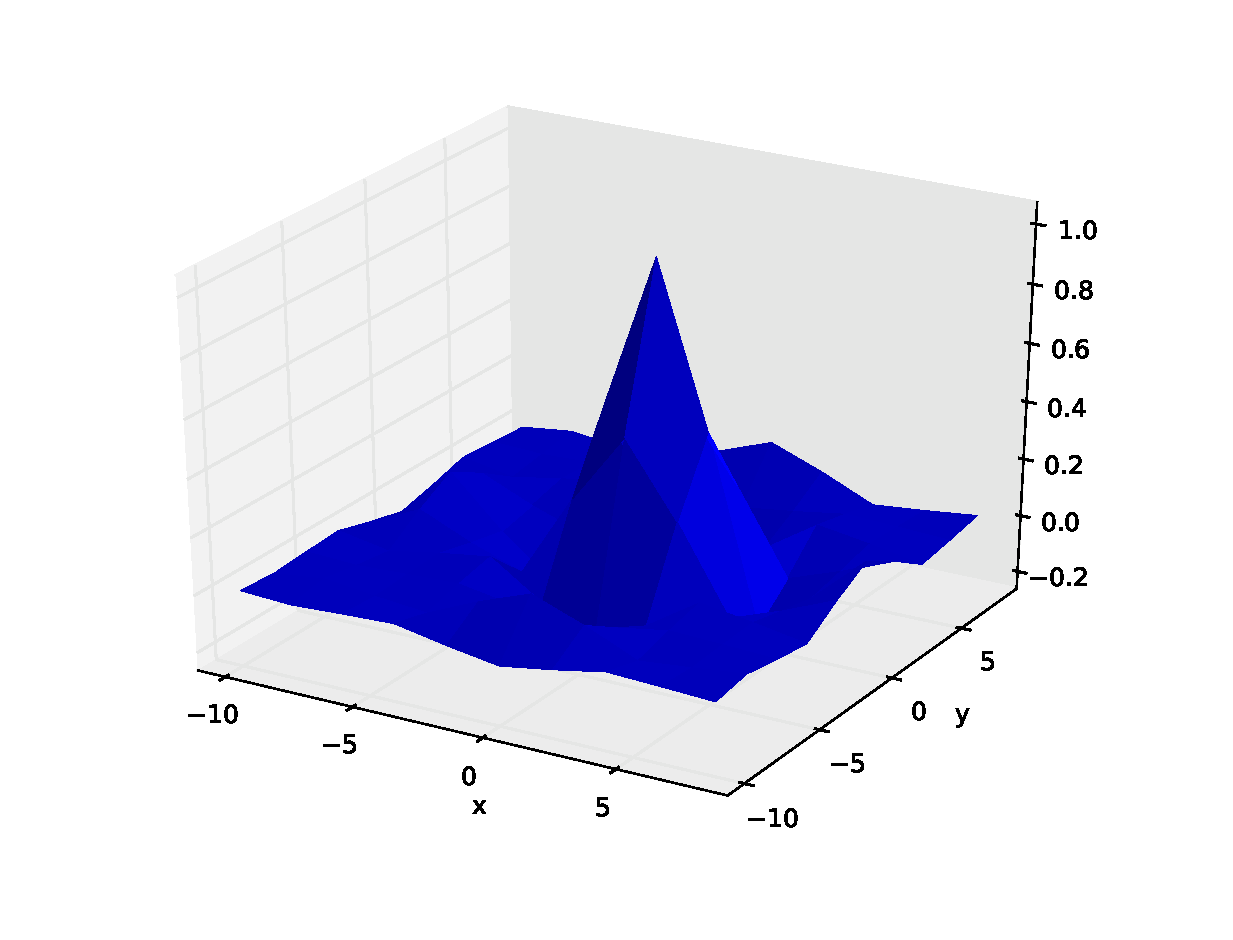
\includegraphics[width = 5cm]{badziewia/test.eps}}
        \Rput[c](2.5,4){\small dane testowe}
	
	\Rput[c](2.5,3){$y = \frac{\sin (x_1) \sin (x_2)}{x_1x_2}$}
        \pause
        \rput[bl](5,2){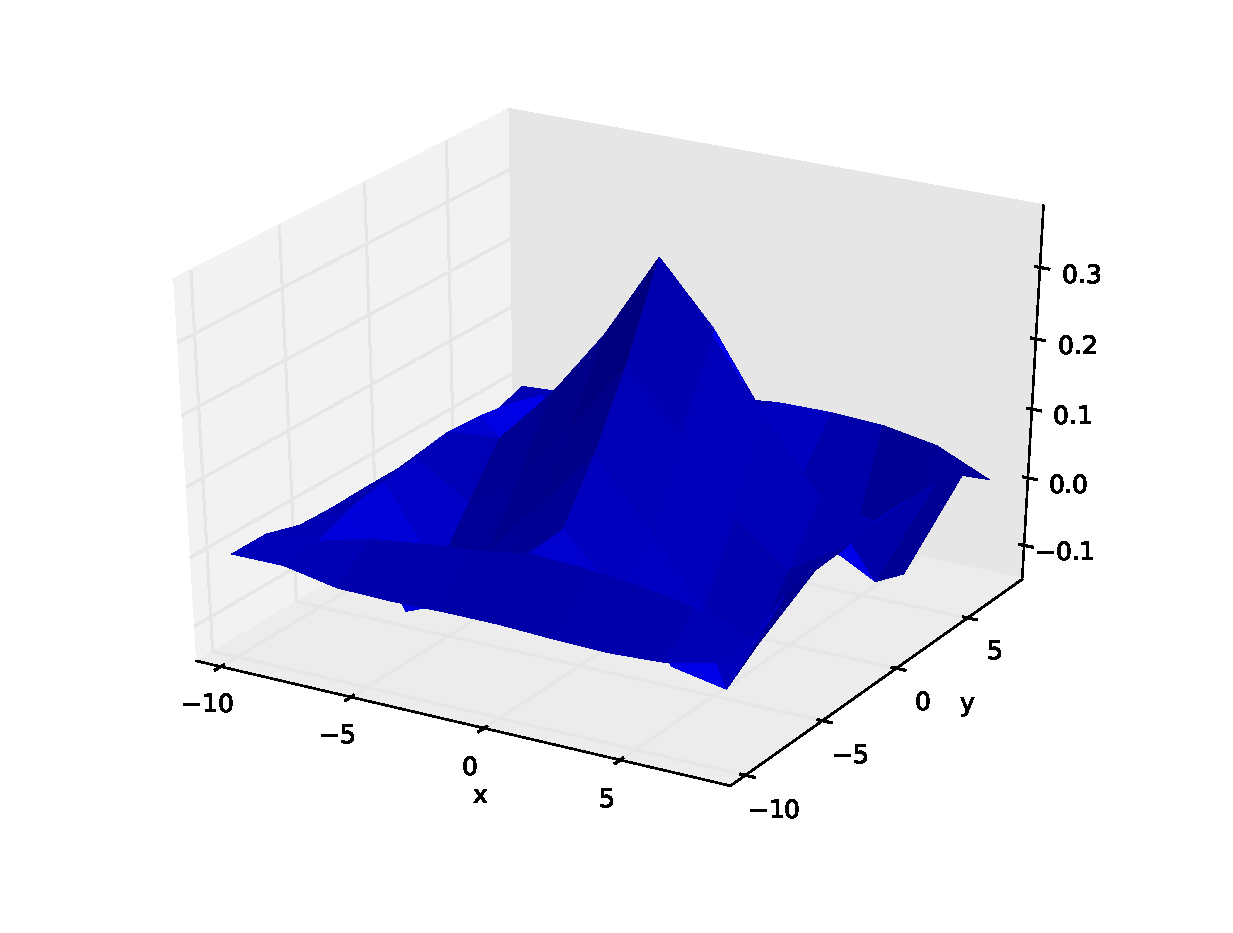
\includegraphics[width = 6cm]{badziewia/lsq.eps}}
        \Rput[c](8,2){\small następniki modelu dostrojone mnk}
\end{pspicture}
}
\frame{
\frametitle{Przykład I}
\begin{pspicture}(18, 8)
        %\psgrid
        \rput[br](11,1.5){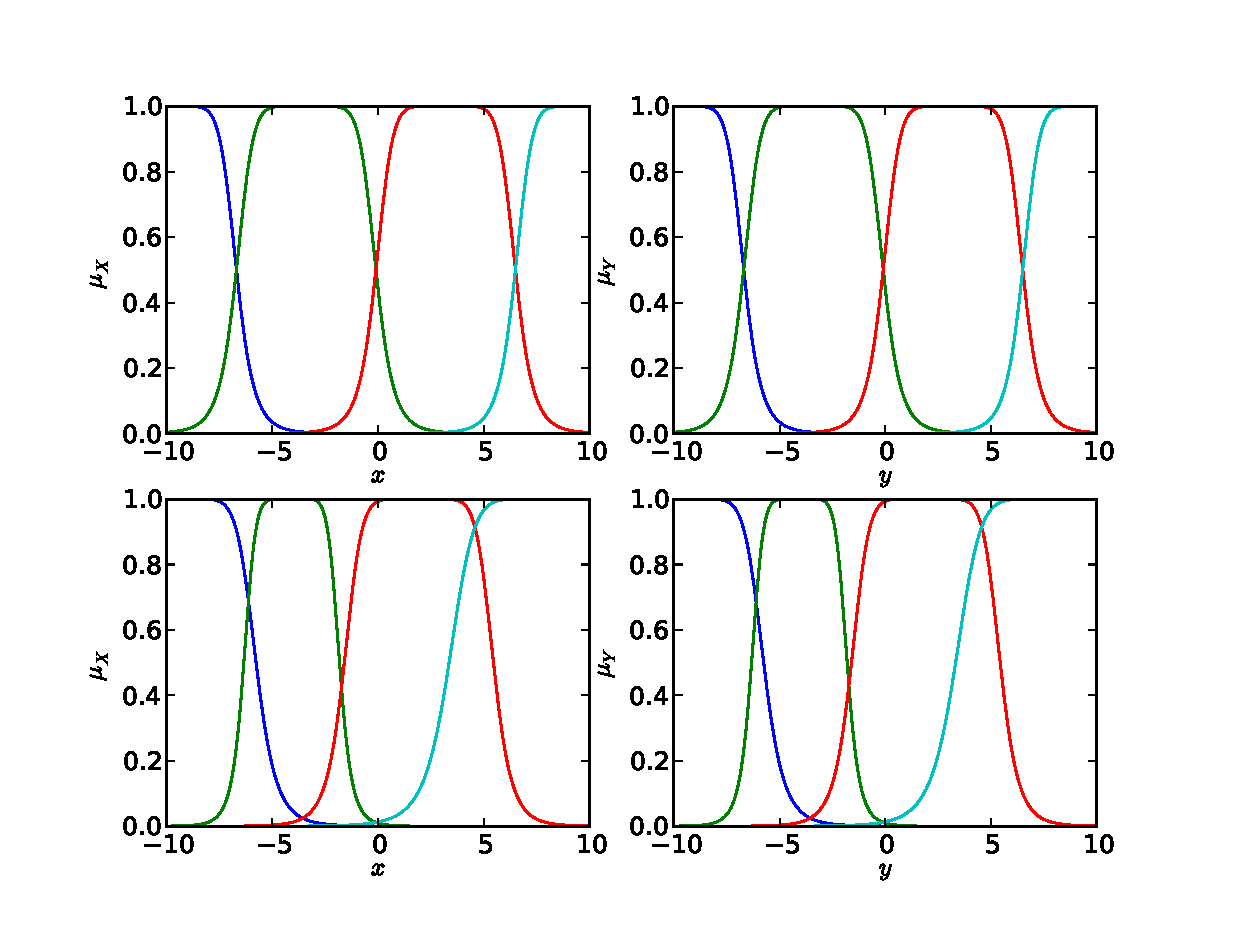
\includegraphics[width = 8cm]{badziewia/memfunc.eps}}
        \Rput[c](6,7.4){\small funkcje przynależności}
        \Rput[r](3.4,5.9){\small sieć nie uczona}
        \Rput[r](3.4,3.1){\small 30 epok uczenia}
\end{pspicture}
}
\frame{
\frametitle{Przykład I}
\begin{pspicture}(18,8)
        %\psgrid
        \rput[bl](0,4){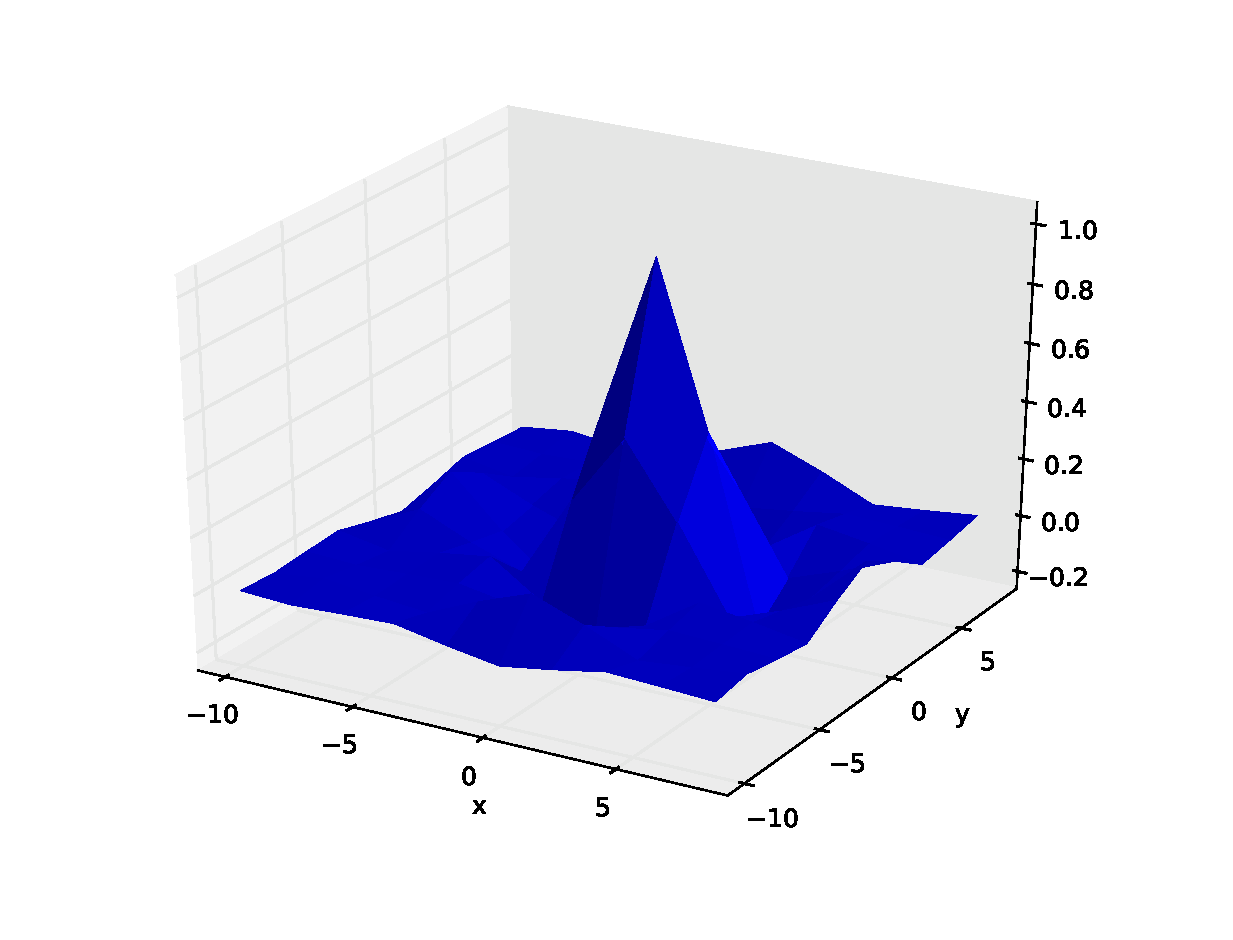
\includegraphics[width = 5cm]{badziewia/test.eps}}
        \Rput[c](2.5,4){\small dane testowe}
        \rput[bl](5,2){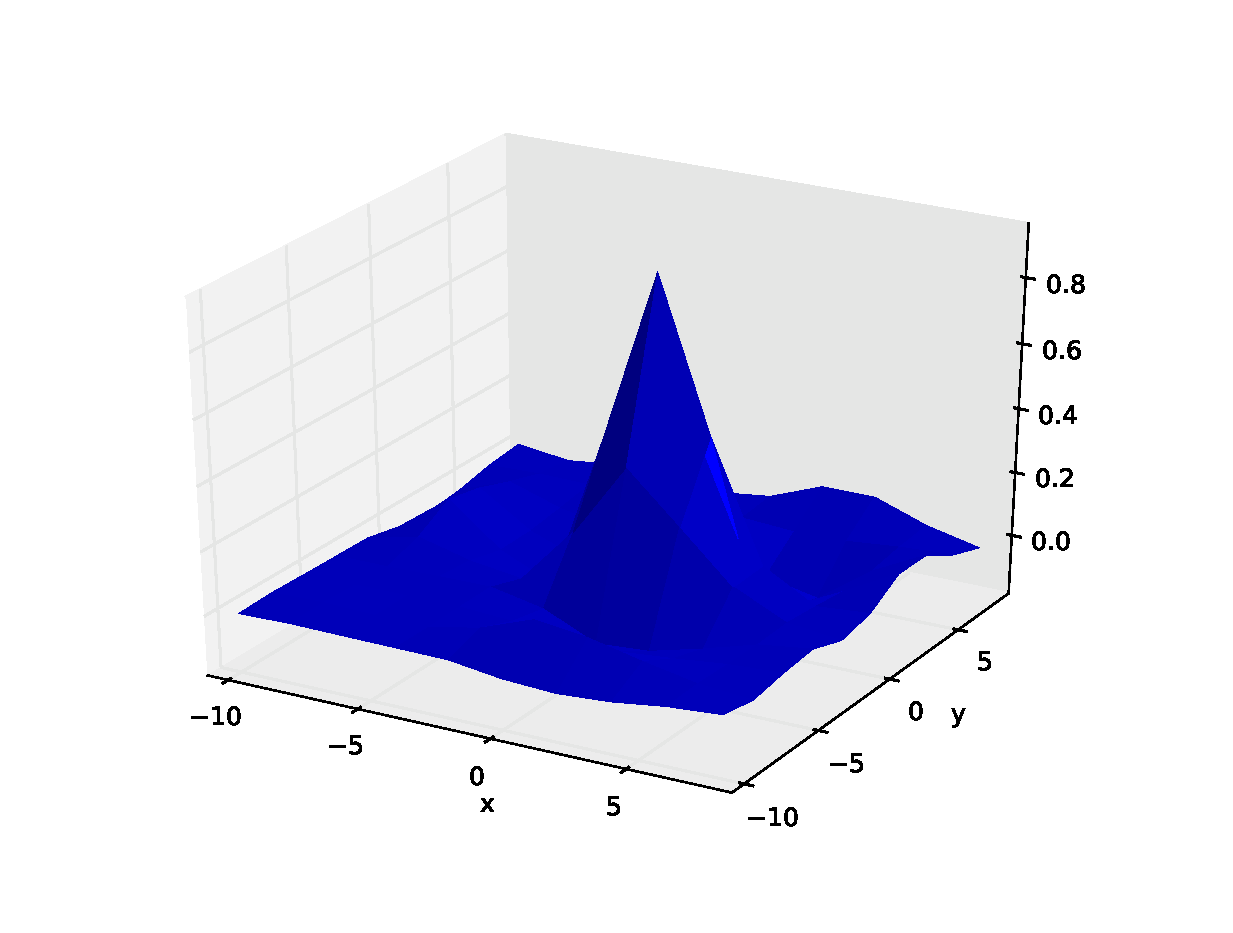
\includegraphics[width = 6cm]{badziewia/train.eps}}
        \Rput[c](8,2){\small 30 epok uczenia}
\end{pspicture}
}
\frame{
\frametitle{Przykład I}
\begin{pspicture}(18,8)
        %\psgrid
        \rput[bl](0,2){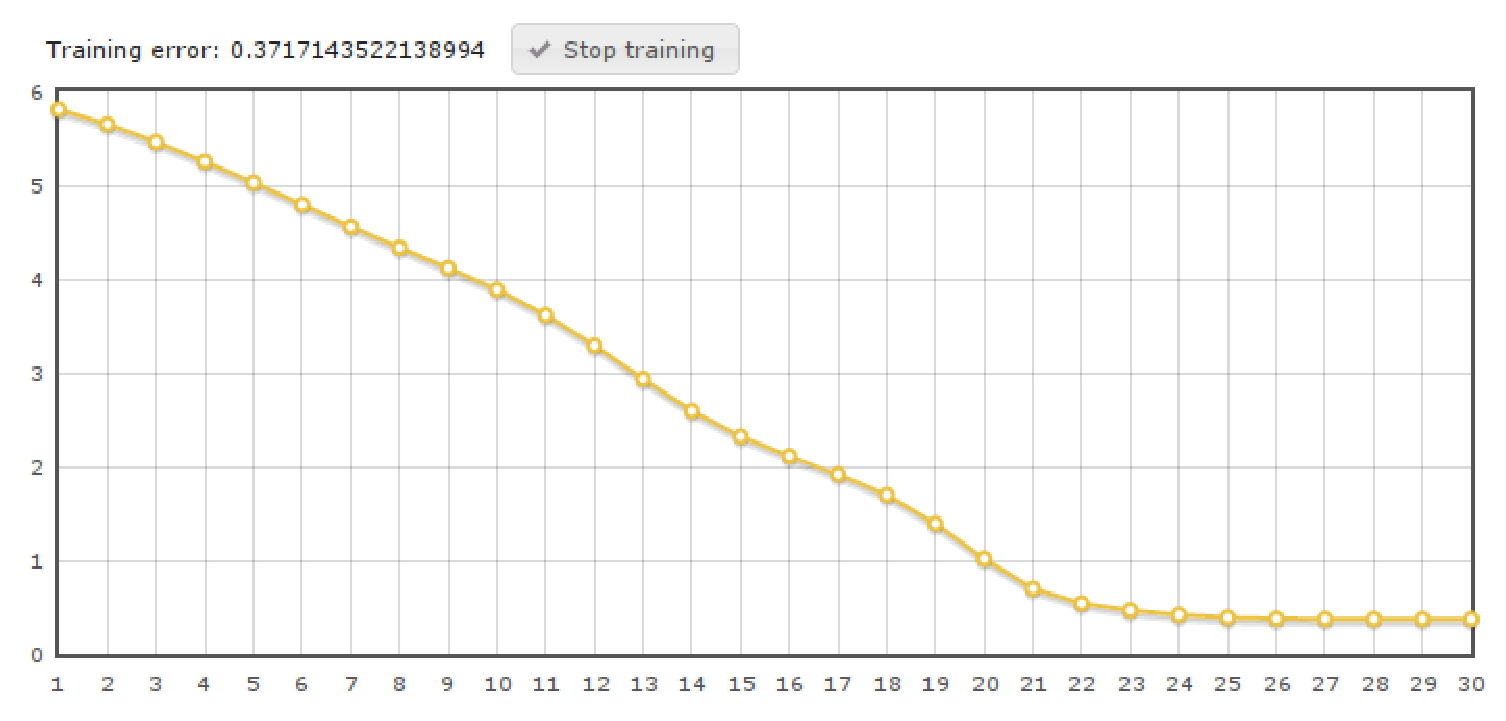
\includegraphics[width = \textwidth]{badziewia/normal.eps}}
\end{pspicture}
}

\frame{
\frametitle{Przykład II}
$y(i) = \sqrt{x(i)} - 0.5 \sin (y(i-1)) + 0.4 y(i-2)$ \\
\small
model rozmyty: 3 wejścia po dwie dzwonowe funkcje przynależności, 8 reguł
\begin{pspicture}(18,8)
        %\psgrid
        \rput[bl](1,2.7){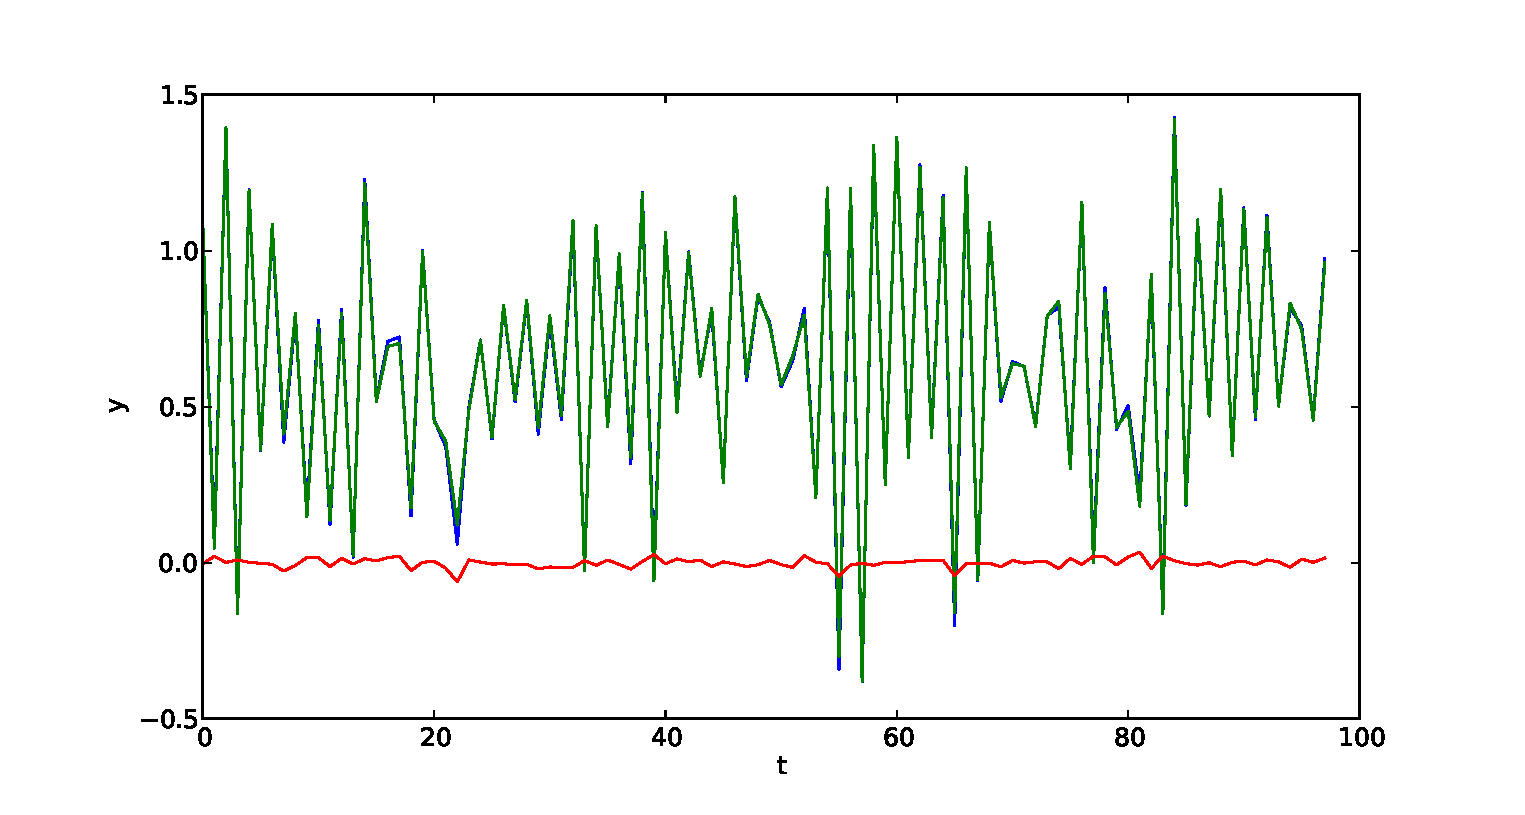
\includegraphics[width = .9\textwidth]{badziewia/dyn.eps}}
\end{pspicture}
}

\section{Algorytmy ewolucyjne w strojeniu modeli rozmytych}
\frame{
\frametitle{Algorytmy ewolucyjne}
\begin{itemize}
\item Ewolucja sztucznych osobników należących do populacji
\item Mutacje
\item Rozmnażanie poprzez krzyżowanie
\item Dobór naturalny
\end{itemize}
}

\frame{
  \frametitle{Algorytmy ewolucyjne w strojeniu modeli rozmytych}
  \begin{itemize}
    \item System rozmyty reprezentowany poprzez wektor genotypu
    \item Genotyp $c$ -- wektor parametrów poprzedników systemu
    \item Następniki zawsze dostrajane metodą najmniejszych kwadratów
\end{itemize}
}

\frame{
\frametitle{Mutacja -- mutacja nierównomierna}
        \begin{displaymath}
            \begin{array}{c}
                c^{l+1} = \left\{ \begin{array}{l} c^{l} + \Delta (l, \delta _{c_{\mathrm{max}}}),\quad b = 0 \\
                                                    c^{l} - \Delta (l, \delta _{c_{\mathrm{max}}}),\quad b = 1
                            \end{array} \right. \\
            \Delta (l,y) = y(1-r^{(1-\frac{l}{l_{\mathrm{max}}})^b})
            \end{array}
        \end{displaymath}
\begin{itemize}
\item $\delta _{c_{\mathrm{max}}}$ - wektor maksymalnych zmian genotypu
\item $b$ - liczba losowa ze zbioru $\{0,1\}$
\item $r$ - liczba losowa z przedziału $[0, 1]$
\item $l$, $l_{\mathrm{max}}$ - numer pokolenia, liczba pokoleń
\end{itemize}

\textbf{Wielkość mutacji maleje w kolejnych pokoleniach}
}

\frame{
\frametitle{Krzyżowanie}
        \begin{displaymath}
            \begin{array}{ll}
            C_1^{l+1} = aC_r^l + (1-a)C_s^l,& C_2^{l+1} = (1-a)C_r^l + aC_s^l,\\
            C_3^{l+1} = \mathrm{min}(C_r^l, C_s^l),& C_4^{l+1} = \mathrm{max}(C_r^l, C_s^l)
            \end{array}
        \end{displaymath}
\begin{itemize}
\item max, min - ekstremum po współrzędnych
\item $a$ - liczba losowa z przedziału $[0,1]$
\end{itemize}
}

\frame{
\frametitle{Dobór naturalny}
\begin{itemize}
\item Ruletka -- prawdopodobieństwo wylosowania odwrotnie proporcjonalne do wartości błędu
\item Możliwe strategie ewolucyjne:
\begin{itemize}
\item $\mu , \lambda$ - przeżywają tylko osobniki z populacji potomnej
\item $\mu + \lambda$ - przeżywają osobniki z populacji potomnej i rodzicielskiej
\end{itemize}
\end{itemize}
}

\frame{
\frametitle{Przykład III}
Dane z przykładu I
\begin{pspicture}(18,8)
        %\psgrid
        \rput[bl](0,2.7){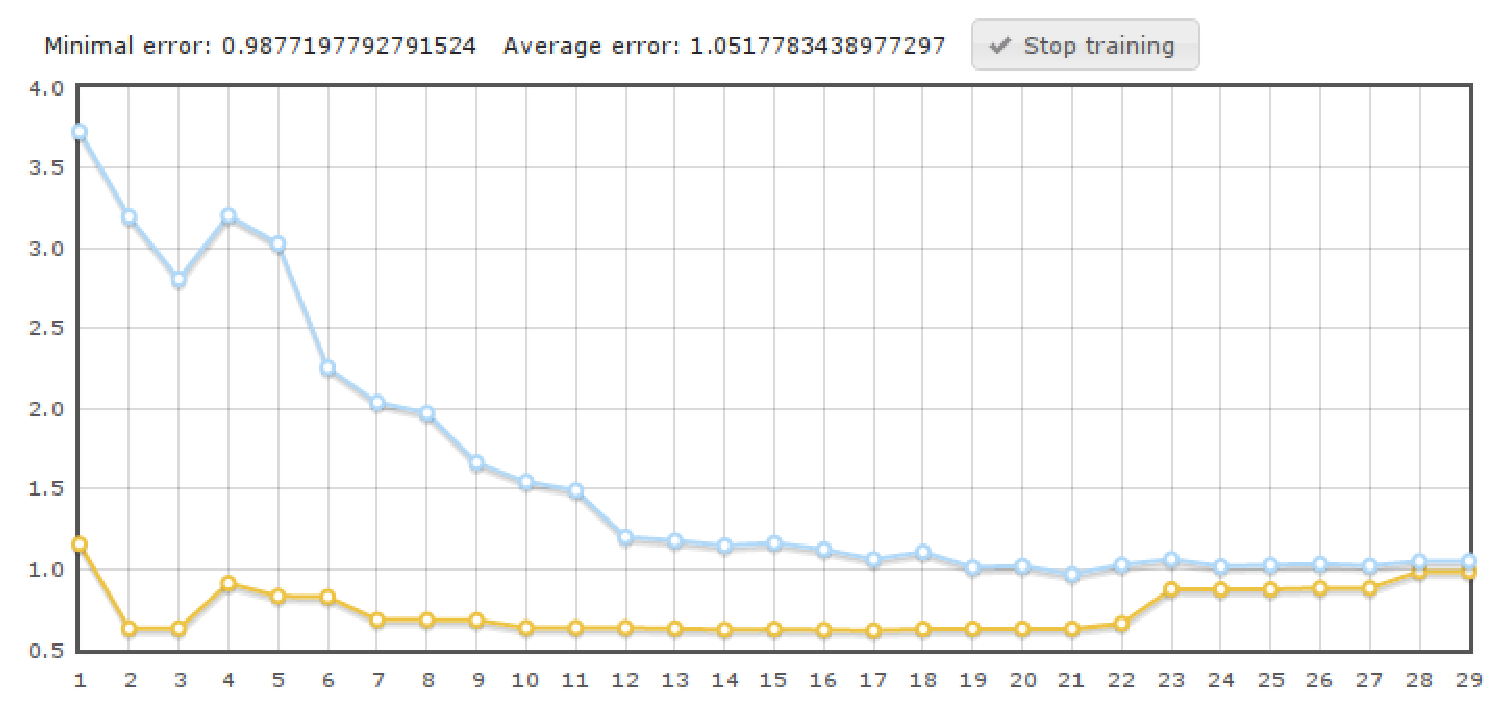
\includegraphics[width = \textwidth]{badziewia/evo.eps}}
\end{pspicture}

}

\section{Implementacja}
\frame{
  \frametitle{Implementacja}
  \begin{itemize}
    \item Wygodne i uniwersalne API do tworzenia i strojenia modeli rozmytych
    \item Elastyczność - swoboda wyboru struktury i parametrów dostrajalnych modelu
    \item Interfejs graficzny oparty o przeglądarkę
    \item Możliwość importu i eksportu danych wykorzystywanych przez MATLAB Fuzzy Toolbox
    \item Wykorzystywane technologie: Python, NumPy, SciPy, Flask, RabbitMQ
  \end{itemize}
}

\subsection{Biblioteka}
\frame{
\frametitle{Interfejs programisty}
3 moduły Pythona:
\begin{itemize}
\item \texttt{pyfis.struct} -- Obiektowa struktura modeli rozmytych TSK
\item \texttt{pyfis.anfis} -- Algorytmy neuronowe strojenia modeli rozmytych
\item \texttt{pyfis.evofis} -- Algorytmy ewolucyjne strojenia modeli rozmytych
\end{itemize}
}

\frame{
\frametitle{Interfejs użytkownika}
\small
\verbatiminput{demo.py}
}

\subsection{Architektura}
\frame{
\frametitle{Architektura}
\begin{itemize}
\item Interfejs oparty o przeglądarkę
\item Długotrwałe zadania obliczeniowe uruchamiane w zewnętrznych procesach
\item Komunikacja procesów poprzez protokół AMQP
\item Dane składowane w relacyjnej bazie danych
\end{itemize}
}

\frame{
\frametitle{Architektura}
\resizebox{\textwidth}{!}{
    \begin{pspicture}(18,10)
    %\psgrid
    \psline[linearc=.5](14,5)(18,5)(18,1)(13,1)(13,5)(14,5)
    \rput[bl](13.5,5.1){PRZEGLĄDARKA}
    \rput[b](15.5,3.2){HTML5}
    \rput[t](15.5,2.8){jQuery}
    \psline[linearc=.5](2,9)(8,9)(8,1)(1,1)(1,9)(2,9)
    \rput[bl](1.5,9.2){SERWER}
    \psline(8,7)(5,7)(5,3)(8,3)
    \rput[bl](5,7.2){Apache, mod\_wsgi}
    \rput[c](6.5,5){Flask}
    \psline(1.75,6)(2.25,6)(2.25,2.75)(1.75,2.75)(1.75,6)
    \pscurve{->}(5,6)(2.25,6.5)(2,6)
    \rput[t](2,2.75){pyfis}
    \psline{->}(2.25,3.5)(5,5)
    \psline{->}(5,4.5)(2.25,3)
    \psline{->}(8,5.25)(13,3.25)
    \psline{->}(13,2.75)(8,4.75)
    \rput[c](10.5, 4){\psframebox*{JSON over HTTP}}
    \rput[c](3.75, 4.2){\psframebox*{AMQP}}
    \end{pspicture}
}
}

\section{Demo}
\frame{
\frametitle{Demo}
}
\frame{
\frametitle{Zadania}
\begin{itemize}
\item Eksport modeli do MATLABa
\item Automatyczne generowanie struktury modeli
\item Modyfikacje algorytmu ewolucyjnego
\item Zwiększenie szybkości działania aplikacji
\end{itemize}
}

\frame{
\begin{center}
  \Large
  Dziękuję za uwagę
\end{center}
}
\end{document}

